% BHU PYQ -- Professional Exam Template
\documentclass[11pt,a4paper]{article}

\usepackage[a4paper,top=2.5cm,bottom=2.5cm,left=2.8cm,right=2.8cm,headheight=14pt]{geometry}
\usepackage{amsmath,amssymb}
\usepackage[T1]{fontenc}
\usepackage[utf8]{inputenc}
\usepackage{lmodern}
\usepackage{microtype}
\usepackage{fancyhdr}
\usepackage{enumitem}
\usepackage{hyperref}
\usepackage{lastpage}
\usepackage{parskip}
\usepackage{tikz}
\usetikzlibrary{arrows.meta,shapes,positioning}

\hypersetup{colorlinks=true,urlcolor=black,linkcolor=black,
  pdftitle={B.Sc. (Hons.) Zoology Sem-III ZOB-301 -- BHU PYQ}}

\pagestyle{fancy}
\fancyhf{}
\renewcommand{\headrulewidth}{0.4pt}
\renewcommand{\footrulewidth}{0.4pt}
\fancyhead[L]{\small   \textit{Banaras Hindu University}}
\fancyhead[R]{\small   \textit{Zoology Paper: ZOB-301}}
\fancyfoot[C]{\small Page  \thepage\ of \pageref{LastPage}}


\newlist{parts}{enumerate}{2}
\setlist[parts,1]{label=(\alph*),leftmargin=*,itemsep=4pt,topsep=3pt}
\setlist[parts,2]{label=(\roman*),leftmargin=*,itemsep=2pt,topsep=2pt}

\newcommand{\pts}[1]{\hfill   \textit{[#1]}}


\begin{document}


\begin{center}
  {\large\bfseries BANARAS HINDU UNIVERSITY}\\[2pt]
  {
\normalsize B.Sc. (Hons.) Semester III Examination, 2023-24}\\[6pt]
  \rule{0.8\linewidth}{0.5pt}\\[6pt]
  {\large\bfseries Zoology}\\[4pt]
  {\large\bfseries Paper: ZOB-301 --- Basic Genetics and Evolution and Developmental Biology}\\[4pt]
  {
\normalsize Time: Three hours \hfill Full Marks: 70}
\end{center}

\rule{\linewidth}{0.4pt}

\smallskip



\noindent   \textit{Note: Answer three questions from Section-A and three questions from Section-B. Question No. 1 in both sections is compulsory. Use a separate answer book for each section. The figures in the right-hand margin indicate marks.}

\bigskip

\begin{center}
   \textbf{SECTION -- A} \\
   \textbf{(Basic Genetics and Evolution) (Marks: 35)}
\end{center}

\medskip


\noindent   \textbf{Question 1.} Answer the following parts:

\begin{parts}
  \item Select and write the best option from the following:\pts{$4  \times \frac{1}{2} = 2$}
  
\begin{parts}
    \item A cross was made between three unlinked genes, $AaBbCc  \times AaBbCc$. What would be the frequency of $AABBCC$ individuals?
    
\begin{parts}
      \item $1/64$
      \item $1/32$
      \item $1/16$
      \item $1/8$
    \end{parts}
    
    \item The phenomenon of `independent assortment' is associated with:
    
\begin{parts}
      \item linked genes
      \item inheritance of genes located on different chromosomes
      \item monohybrid cross
      \item location of chromosomes in an interphase cell
    \end{parts}
    
    \item If the blood group of the mother is A and the blood group of the father is B, then the blood group of children could be:
    
\begin{parts}
      \item A, AB only
      \item A, B, AB, O
      \item B, AB only
      \item O, A, B only
    \end{parts}
    
    \item Which of the following statements describes Epistasis?
    
\begin{parts}
      \item An allele that changes the genotype of another allele
      \item A gene that changes the genotype of another gene
      \item A gene that masks the expression of another gene
      \item An allele that masks the expression of another allele
    \end{parts}
  \end{parts}

  \item Write whether the following statements are True or False giving reasons in 2--3 sentences each:\pts{$2  \times 2 = 4$}
  
\begin{parts}
    \item Darwin finches are examples of adaptive radiation.
    \item Monohybrid crosses revealed the phenomenon of incomplete dominance.
  \end{parts}

  \item Differentiate between penetrance and expressivity.\pts{$2$}

  \item Match the terms in Column-X with Column-Y:\pts{$6  \times \frac{1}{2} = 3$}
  
\begin{center}
    \renewcommand{\arraystretch}{1.2}
    
\begin{tabular}{llp{0.5cm}ll}
      \hline
   \textbf{Column-X} & & &   \textbf{Column-Y} \\
      \hline
      (i) Pericentric inversion & & & (1) Phenocopy \\
      (ii) Wing of a bird and wing of an insect & & & (2) Coiling of snail shell \\
      (iii) Remnant of ancient animals & & & (3) Epistasis \\
      (iv) Natural selection & & & (4) Analogous organ \\
      (v) Sodium metaborate & & & (5) Chromosome \\
      (vi) Maternal inheritance & & & (6) Translocation \\
      & & & (7) Darwin \\
      & & & (8) Fossil \\
      \hline
    \end{tabular}
  \end{center}
\end{parts}

\medskip


\noindent   \textbf{Question 2.} Answer the following parts:

\begin{parts}
  \item ``Increase and decrease in individual chromosome number in an individual can cause syndromes.'' Justify the statement with examples.\pts{$4$}
  \item Differentiate between the evolutionary theories of Lamarck and Darwin.\pts{$4$}
  \item One variety of plant having leaves with cuts on them was crossed with plants having normal leaves. All the F1 progeny produced cut leaves. Two of the F1 plants were interbred to produce F2. The F2 had 248 cut leaves and 16 normal leaves. Describe the phenomenon that determines the leaf pattern.\pts{$4$}
\end{parts}

\medskip


\noindent   \textbf{Question 3.} Answer the following parts:

\begin{parts}
  \item The pedigree represents the pattern of inheritance. Look at the pedigree and answer the following:\pts{$6$}
  
\begin{parts}
    \item Which type of inheritance is it, dominant or recessive? Justify.
    \item Is it autosomal or sex-linked? Justify.
  \end{parts}
  
  
\begin{center}
  
\begin{tikzpicture}[
    scale=0.85,
    male/.style={rectangle, draw, minimum size=0.5cm, inner sep=0pt, thick},
    female/.style={circle, draw, minimum size=0.5cm, inner sep=0pt, thick},
    affected_male/.style={rectangle, draw, fill=black, minimum size=0.5cm, inner sep=0pt, thick},
    affected_female/.style={circle, draw, fill=black, minimum size=0.5cm, inner sep=0pt, thick}
  ]
    % Generation I
    
ode[male] (I1) at (-0.5, 0) {}; 
ode[below=2pt] at (I1) {1};
    
ode[female] (I2) at (1.0, 0) {}; 
ode[below=2pt] at (I2) {2};
    \draw[thick] (I1) -- (I2);
    \coordinate (I_mid) at (0.25, 0);
  
    % Generation II
    
ode[affected_male] (II1) at (-4.5, -1.8) {}; 
ode[below=2pt] at (II1) {1};
    
ode[male] (II2) at (-3.0, -1.8) {}; 
ode[below=2pt] at (II2) {2};
    
ode[female] (II3) at (-1.5, -1.8) {}; 
ode[below=2pt] at (II3) {3};
    
ode[female] (II4) at (0.5, -1.8) {}; 
ode[below=2pt] at (II4) {4};
    
ode[female] (II5) at (2.0, -1.8) {}; 
ode[below=2pt] at (II5) {5};
    
ode[affected_male] (II6) at (3.5, -1.8) {}; 
ode[below=2pt] at (II6) {6};
    
ode[male] (II7) at (5.0, -1.8) {}; 
ode[below=2pt] at (II7) {7};
  
    % Connect Generation I to II
    \draw[thick] (I_mid) -- (0.25, -1.0);
    \draw[thick] (-4.5, -1.0) -- (5.0, -1.0);
    \draw[thick] (-4.5, -1.0) -- (II1);
    \draw[thick] (-3.0, -1.0) -- (II2);
    \draw[thick] (0.5, -1.0) -- (II4);
    \draw[thick] (2.0, -1.0) -- (II5);
    \draw[thick] (5.0, -1.0) -- (II7);
  
    % Marriage II-2 x II-3
    \draw[thick] (II2) -- (II3);
    \coordinate (II_2_3_mid) at (-2.25, -1.8);
  
    % Marriage II-5 x II-6
    \draw[thick] (II5) -- (II6);
    \coordinate (II_5_6_mid) at (2.75, -1.8);
  
    % Generation III
    
ode[affected_male] (III1) at (-4.0, -3.6) {}; 
ode[below=2pt] at (III1) {1};
    
ode[female] (III2) at (-2.5, -3.6) {}; 
ode[below=2pt] at (III2) {2};
    
ode[male] (III3) at (-1.8, -3.6) {}; 
ode[below=2pt] at (III3) {3};
    
ode[affected_male] (III4) at (-0.5, -3.6) {}; 
ode[below=2pt] at (III4) {4};
  
    
ode[male] (III5) at (1.0, -3.6) {}; 
ode[below=2pt] at (III5) {5};
    
ode[male] (III6) at (2.0, -3.6) {}; 
ode[below=2pt] at (III6) {6};
    
ode[male] (III7) at (3.0, -3.6) {}; 
ode[below=2pt] at (III7) {7};
    
ode[male] (III8) at (4.0, -3.6) {}; 
ode[below=2pt] at (III8) {8};
    
ode[female] (III9) at (5.0, -3.6) {}; 
ode[below=2pt] at (III9) {9};
    
ode[male] (III10) at (6.5, -3.6) {}; 
ode[below=2pt] at (III10) {10};
  
    % Connect II-2/3 to III-1, 3, 4
    \draw[thick] (II_2_3_mid) -- (-2.25, -2.7);
    \draw[thick] (-4.0, -2.7) -- (-0.5, -2.7);
    \draw[thick] (-4.0, -2.7) -- (III1);
    \draw[thick] (-1.8, -2.7) -- (III3);
    \draw[thick] (-0.5, -2.7) -- (III4);
  
    % Connect II-5/6 to III-5, 6, 7, 8, 9
    \draw[thick] (II_5_6_mid) -- (2.75, -2.7);
    \draw[thick] (1.0, -2.7) -- (5.0, -2.7);
    \draw[thick] (1.0, -2.7) -- (III5);
    \draw[thick] (2.0, -2.7) -- (III6);
    \draw[thick] (3.0, -2.7) -- (III7);
    \draw[thick] (4.0, -2.7) -- (III8);
    \draw[thick] (5.0, -2.7) -- (III9);
  
    % Marriage III-1 x III-2
    \draw[thick] (III1) -- (III2);
    \coordinate (III_1_2_mid) at (-3.25, -3.6);
  
    % Marriage III-9 x III-10
    \draw[thick] (III9) -- (III10);
    \coordinate (III_9_10_mid) at (5.75, -3.6);
  
    % Generation IV
    
ode[female] (IV1) at (-4.6, -5.4) {}; 
ode[below=2pt] at (IV1) {1};
    
ode[male] (IV2) at (-3.9, -5.4) {}; 
ode[below=2pt] at (IV2) {2};
    
ode[male] (IV3) at (-3.2, -5.4) {}; 
ode[below=2pt] at (IV3) {3};
    
ode[female] (IV4) at (-2.5, -5.4) {}; 
ode[below=2pt] at (IV4) {4};
    
ode[male] (IV5) at (-1.8, -5.4) {}; 
ode[below=2pt] at (IV5) {5};
  
    
ode[female] (IV6) at (4.0, -5.4) {}; 
ode[below=2pt] at (IV6) {6};
    
ode[male] (IV7) at (4.8, -5.4) {}; 
ode[below=2pt] at (IV7) {7};
    
ode[female] (IV8) at (5.6, -5.4) {}; 
ode[below=2pt] at (IV8) {8};
    
ode[affected_male] (IV9) at (6.4, -5.4) {}; 
ode[below=2pt] at (IV9) {9};
  
    % Connect III-1/2 to IV-1 to 5
    \draw[thick] (III_1_2_mid) -- (-3.25, -4.5);
    \draw[thick] (-4.6, -4.5) -- (-1.8, -4.5);
    \draw[thick] (-4.6, -4.5) -- (IV1);
    \draw[thick] (-3.9, -4.5) -- (IV2);
    \draw[thick] (-3.2, -4.5) -- (IV3);
    \draw[thick] (-2.5, -4.5) -- (IV4);
    \draw[thick] (-1.8, -4.5) -- (IV5);
  
    % Connect III-9/10 to IV-6 to 9
    \draw[thick] (III_9_10_mid) -- (5.75, -4.5);
    \draw[thick] (4.0, -4.5) -- (6.4, -4.5);
    \draw[thick] (4.0, -4.5) -- (IV6);
    \draw[thick] (4.8, -4.5) -- (IV7);
    \draw[thick] (5.6, -4.5) -- (IV8);
    \draw[thick] (6.4, -4.5) -- (IV9);
  
    % Generation labels
    
ode[left=1.5cm] at (I1) {   \textbf{I}};
    
ode[left=0.8cm] at (II1) {   \textbf{II}};
    
ode[left=1.2cm] at (III1) {   \textbf{III}};
    
ode[left=1.5cm] at (IV1) {   \textbf{IV}};
  \end{tikzpicture}
  \end{center}

  \item Write short notes on the following:\pts{$2  \times 3 = 6$}
  
\begin{parts}
    \item Antibiotic resistance in bacteria
    \item Chromosomal basis of sex determination
  \end{parts}
\end{parts}

\medskip


\noindent   \textbf{Question 4.} Answer the following parts:

\begin{parts}
  \item What is Neo-Darwinism and Modern Synthesis of Evolution and how it has redefined the old theory?\pts{$4$}
  \item Chromosome 1 of an individual undergoes paracentric inversion. What will be the consequences of meiosis in case crossing-over occurs in the inverted part of chromosomes in a heterozygous condition? Write the answers with the help of diagrams.\pts{$6$}
  \item A box has 8 red, 7 blue and 6 green balls. If one ball is picked up randomly, what is the probability that it is neither red nor green?\pts{$2$}
\end{parts}

\pagebreak

\begin{center}
   \textbf{SECTION -- B} \\
   \textbf{(Developmental Biology) (Marks: 35)}
\end{center}

\medskip


\noindent   \textbf{Question 1.} Answer the following parts:

\begin{parts}
  \item Define the following:\pts{$5  \times 1 = 5$}
  
\begin{parts}
    \item Regeneration blastema
    \item Morula
    \item Spermiogenesis
    \item Koller's sickle
    \item Yolk plug
  \end{parts}

  \item Differentiate between the following:\pts{$3  \times 2 = 6$}
  
\begin{parts}
    \item Preformation and Epigenesis
    \item Radial cleavage and Spiral cleavage
    \item Autonomous specification and Syncytial specification
  \end{parts}
\end{parts}

\medskip


\noindent   \textbf{Question 2.} Answer the following parts:

\begin{parts}
  \item Give an illustrated account of external fertilization in sea urchin.\pts{$10$}
  \item Write a brief note on the functions of egg membranes.\pts{$2$}
\end{parts}

\medskip


\noindent   \textbf{Question 3.} Answer the following parts:

\begin{parts}
  \item Describe the process of three germ layers formation in chick.\pts{$9$}
  \item Draw a well-labelled diagram of the fate map of a frog embryo.\pts{$3$}
  
  
\begin{center}
  
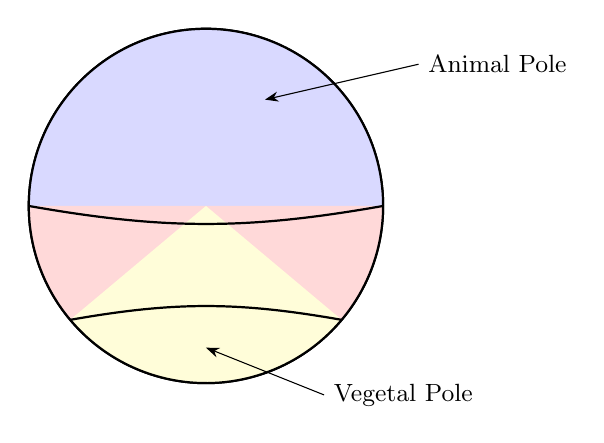
\begin{tikzpicture}[scale=1.5, >=Stealth, every node/.style={font=\small}]
    % Outer boundary
    \draw[thick] (0,0) circle (1.5);
    
    % Fill areas
    % Ectoderm: 0 to 180 degrees
    \fill[blue!15] (0,0) -- (0:1.5) arc (0:180:1.5) -- cycle;
    
    % Mesoderm (Marginal zone)
    \fill[red!15] (0,0) -- (180:1.5) arc (180:220:1.5) to[out=40, in=140] (320:1.5) arc (320:360:1.5) -- cycle;
    
    % Endoderm (Vegetal pole)
    \fill[yellow!15] (0,0) -- (220:1.5) arc (220:320:1.5) -- cycle;
    
    % Overlay borders
    \draw[thick] (0:1.5) arc (0:180:1.5);
    \draw[thick] (180:1.5) arc (180:220:1.5);
    \draw[thick] (320:1.5) arc (320:360:1.5);
    \draw[thick] (220:1.5) arc (220:320:1.5);
    \draw[thick] (180:1.5) to[out=-10, in=190] (0:1.5);
    \draw[thick] (220:1.5) to[out=10, in=170] (320:1.5);
    
    % Labels
    
ode at (0, 0.7) {   \textbf{Ectoderm} (Epidermal/Neural)};
    
ode at (0, -0.2) {   \textbf{Mesoderm} (Notochord/Somites)};
    
ode at (0, -0.9) {   \textbf{Endoderm}};
    
    % Annotation arrows
    \draw[<-] (0.5, 0.9) -- (1.8, 1.2) node[right] {Animal Pole};
    \draw[<-] (0, -1.2) -- (1.0, -1.6) node[right] {Vegetal Pole};
  \end{tikzpicture}
  \end{center}
\end{parts}

\medskip


\noindent   \textbf{Question 4.} Write short notes on the following:\pts{$3  \times 4 = 12$}

\begin{parts}
  \item Molecular responses to thyroid hormones during metamorphosis
  \item Role of Nieuwkoop center in the formation of dorsal-ventral axis in frog
  \item Types of eggs
\end{parts}

\vfill
\rule{\linewidth}{0.4pt}

\begin{center}\small
\href{https://bhu-exam.vercel.app/}{Click Here}\\[4pt]\href{https://me-aryan.vercel.app/}{Click Here}\\[4pt]\href{https://quashan-me.vercel.app/}{Click Here}
\end{center}

\end{document}
